% Author: Rasmus Pank Roulund
% Inspired by figure in:
% Howells, Peter og Bain, Keith (2007). Financial markets and
% institutions. 5. udg. Essex: Pearson Education.
\documentclass{standalone}
\usepackage{tikz}
\usepackage{comment}
\usetikzlibrary{arrows,fit,calc}
\usetikzlibrary{automata}
\usetikzlibrary{trees}
\usetikzlibrary{arrows,positioning} 
\usepackage{eulervm}
\usepackage[osf,sc]{mathpazo}
\usepackage{inconsolata}

\makeatletter
\newenvironment{minsizebox}[2]{%
	\pgfmathsetlength\@tempdima{#2}%
	\pgfmathsetlength\pgf@yc{\pgfkeysvalueof{/pgf/inner ysep}}%
	\advance\@tempdima by -2\pgf@yc
	\begin{lrbox}{\@tempboxa}%
		\begin{minipage}[t]{#1}%
			\vspace{0pt}%
		}{%
	\end{minipage}%
\end{lrbox}%
\ifdim\@tempdima>\dp\@tempboxa
\dp\@tempboxa=\@tempdima
\fi
\box\@tempboxa
}
\makeatother

\tikzset{
    %Define standard arrow tip
    >=stealth',
    %Define style for boxes
    punkt/.style={
           rectangle,
           rounded corners,
           draw=black, very thick,
           text width=6em,
           minimum height=2em,
           text centered},
    % Define arrow style
    pil/.style={
           ->,
           thick,
           shorten <=2pt,
           shorten >=2pt,}
}

\begin{document}

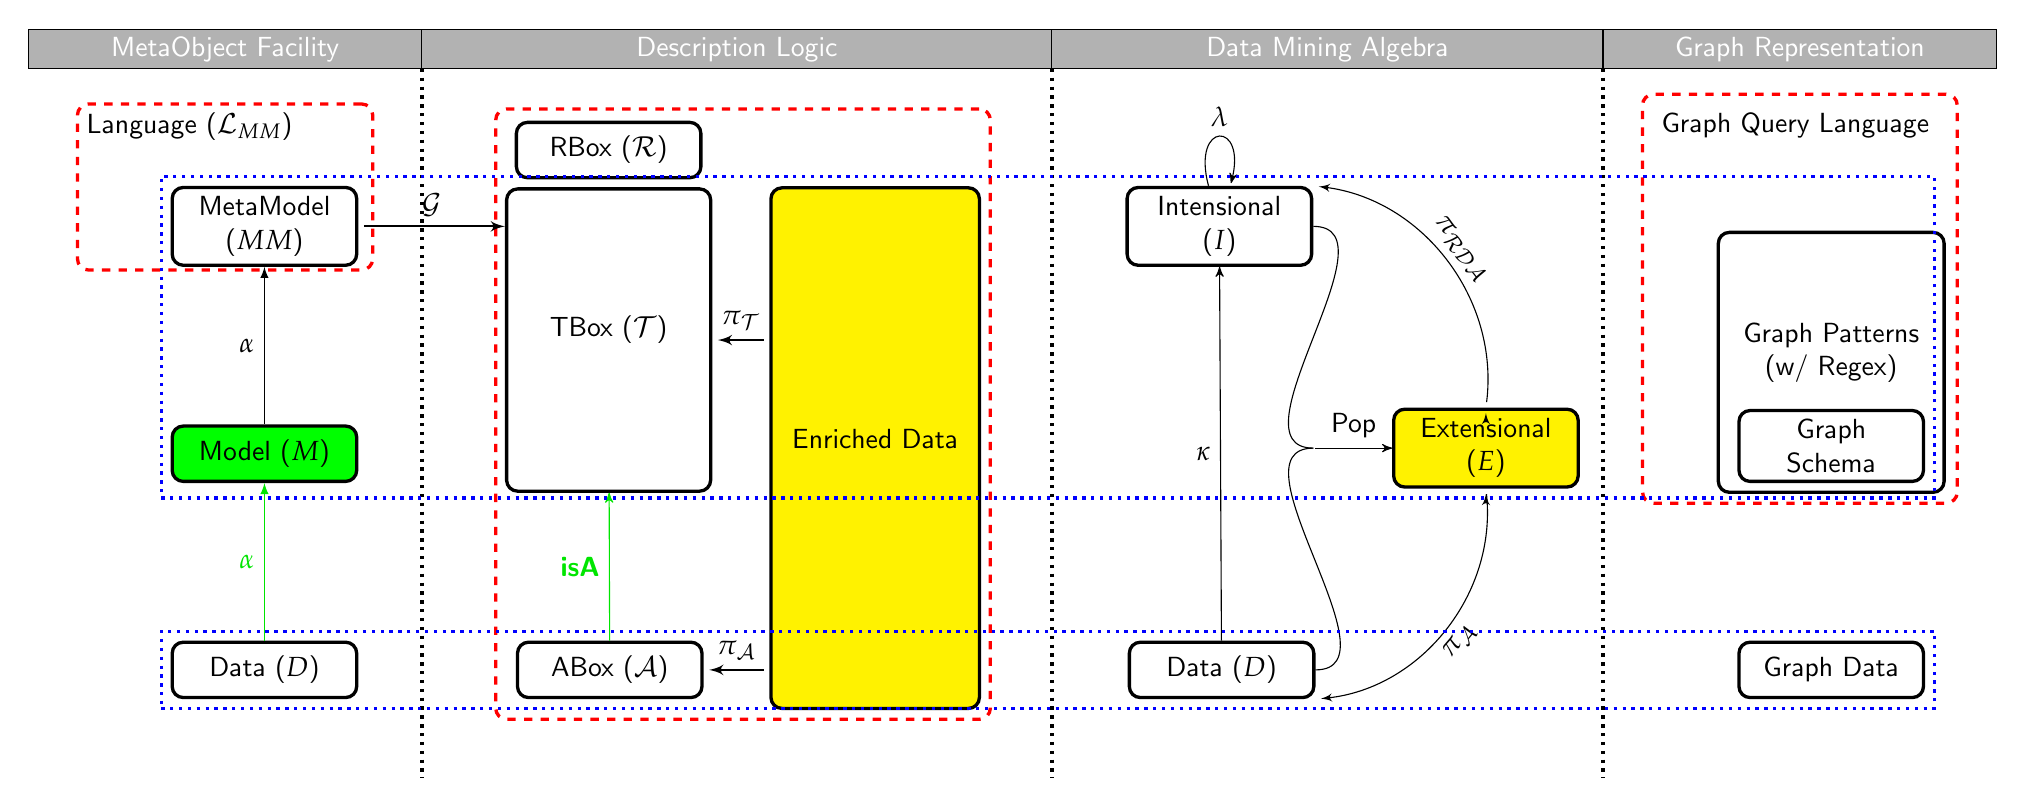
\begin{tikzpicture}[node distance=2cm, auto,font=\sffamily]
 %Modelling
 \draw[fill=black!30] (2,2) rectangle (-3,2.5);
 \node[text=white] at ($(2,2)!.5!(-3,2.5)$) {MetaObject Facility};
 
 %Modelling
 \node[punkt] (mm) {MetaModel ($MM$)};
 \node[punkt,below=of mm,fill=green] (m) {Model ($M$)};
 \node[punkt,below=of m] (d) {Data ($D$)};
 \node[punkt,dashed, text width=10em,minimum height=6em,draw=red] (language) at (-0.5,0.5) {\begin{minsizebox}{12em}{6em}Language ($\mathcal{L}_{MM}$)\end{minsizebox}};
 
 \draw[-latex,draw=green!90!black,text=green!90!black] (d) to node [midway,left] {$\alpha$} (m); 
 \draw[-latex] (m) to node [midway,left] {$\alpha$} (mm); 
 
 
%%%%%
\draw[black,very thick,dotted] (2,2) -- (2,-7);
%%%%%
 
 %Description Logic
 
 \node (rb) at (7,1.25) {};
 \node[text width=6em,minimum height=2em,right =of mm] (tb1) {};
 \node[text width=6em,minimum height=2em,right =of m] (tb2) {};
 \node[punkt,fit=(tb1) (tb2)] (tb) {TBox ($\mathcal{T}$)};
 \node[punkt,right=of d] (ab) {ABox ($\mathcal{A}$)};
 
 
 \node[punkt,above =1mm of tb] (DLF) {RBox ($\mathcal R$)};
 \node[punkt,right=1cm of tb1] (tn2) {};
 \node[punkt,right=1cm of ab] (an2) {};
 \node[punkt,fit=(tn2) (an2),fill=yellow] (ed) {Enriched Data};
 
 \node[punkt, fit=(ab) (tb) (rb) (ed) (DLF),draw=red,dashed,very thick] (DL) {};
  \draw[->,draw=green!90!black,text=green!90!black] (ab) to node [midway,left] {\textbf{isA}} (tb); 
  
  %\draw[->, >=latex', shorten >=2pt, shorten <=2pt, bend left=45,thick,color=red] (language.east) -- node[above,midway,sloped] {$\tau$} ($(DL.south west)!(language.east)!(DL.north west)$);
  
  \draw[->, >=latex', shorten >=2pt, shorten <=2pt, bend left=45,thick] ($(ed.south west)!(tb.east)!(ed.north west)$) -- node[above,midway,sloped] {$\pi_\mathcal{T}$} (tb.east);
  \draw[->, >=latex', shorten >=2pt, shorten <=2pt, bend left=45,thick] ($(ed.south west)!(ab.east)!(ed.north west)$) -- node[above,midway,sloped] {$\pi_\mathcal{A}$} (ab.east);
    
\draw[->, >=latex', shorten <=2pt,% bend left=45,
		thick]  
    (mm.east) to node[midway,above] {$\mathcal G$}($(tb.south west)!(mm)!(tb.north west)$);

%%%%%
\draw[black,very thick,dotted] (10,2) -- (10,-7);
\draw[fill=black!30] (2,2) rectangle (10,2.5);
\node[text=white] at ($(2,2)!.5!(10,2.5)$) {Description Logic};
%%%%%


 
 \node[punkt,right =of an2] (D) {Data ($D$)};
 \node[punkt,right =of tn2] (I) {Intensional ($I$)};
 
 \draw[->] (D) to node [midway,left] {$\kappa$} (I); 
 \path (I) edge [loop above] node[above] {$\lambda$} (I);
  \node[text width=6em,minimum height=2em,right=1cm of D] (D2) {};
  \node[text width=6em,minimum height=2em,right=1cm of I] (I2) {};

  \node[punkt,fill=yellow] at ($(I2)!.5!(D2)$) (E) {Extensional ($E$)};
  
  
  \node[scale=0.1] at ($(I.east)!.5!(D.east)$) (helper) {};
  \draw (I.east) edge[-,out=0,in=180]                  (helper);
  \draw (D.east) edge[-,out=0,in=180]                  (helper);
  \draw[->] (helper) -- node [midway,sloped,above] {Pop} (E);
    
\draw[->, >=latex', shorten >=2pt, shorten <=2pt, bend left=45] (E.north) edge [bend right] node[above,midway,sloped] {$\pi_\mathcal{RDA}$} (I.north east);

\draw[->, >=latex', shorten >=2pt, shorten <=2pt, bend left=45] (E.south) edge [bend left] node[below,midway,sloped] {$\pi_\mathcal{A}$} (D.south east);
    
%%%%%
\draw[black,very thick,dotted] (17,2) -- (17,-7);
\draw[fill=black!30] (10,2) rectangle (17,2.5);
\node[text=white] at ($(10,2)!.5!(17,2.5)$) {Data Mining Algebra};
%%%%%
    
 %\draw[->, >=latex', shorten >=2pt, shorten <=2pt, bend left=45,thick,color=green!60]  
 %   (ed.west) to node[midway,above] {$\alpha_1$}(d.south); 
 %\draw[-latex,color=green!60,thick,shorten >=2pt,shorten <=2pt] (ed) to node [midway,left] {$\alpha_2$} (o); 
 
\node[punkt,right =of D2] (GD) {Graph Data};
\node[punkt,above =of GD] (GS) {Graph Schema};
\node[text width=6em,minimum height=2em,above of=0.5mm GS,fit=(GS)] (Gb) {};
\node[punkt,fit=(GS) (Gb)] (GP) {Graph Patterns (w/ Regex)};
\node[text width=10em,minimum height=6em] (language2) at (19.5,0.5) {\begin{minsizebox}{12em}{6em}Graph Query Language\end{minsizebox}};
\node[punkt,dashed, text width=10em,minimum height=6em,draw=red,fit=(GS)(GP)(language2)] (bu) {}; 
\node[draw=blue,dotted,fit=(d) (GD),very thick] {};
\node[draw=blue,dotted,fit=(mm) (GS) (E),very thick] {};


\draw[fill=black!30] (17,2) rectangle (22,2.5);
\node[text=white] at ($(17,2)!.5!(22,2.5)$) {Graph Representation};
\end{tikzpicture}

\end{document}

%%% Local Variables:
%%% mode: latex
%%% TeX-master: t
%%% End:

